% Source: graduate-coursework/Prior_Semesters/Fa24/EMCH371/assignments/hw2.tex

\documentclass[border=4pt]{standalone}
\usepackage{amsmath}
\usepackage{graphicx}
\usepackage{pgfplots}
\usepackage{tikz}
\pgfplotsset{compat=1.18}
\usetikzlibrary{3d,calc}

\begin{document}
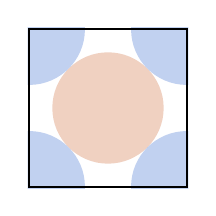
\begin{tikzpicture}
        
        % Define colors for atoms
        \definecolor{atomcorner}{rgb}{0.2, 0.4, 0.8} % Blueish color
        \definecolor{atomcenter}{rgb}{0.8, 0.4, 0.2} % Orangeish color
        
        % Define clipping path for the square
        \clip (-0.02,-0.02) rectangle (2.02,2.02);
        
        % Draw center atom
        \fill[atomcenter, opacity=0.3] (1,1) circle (0.707); % Center atom
        
        % Draw corner atoms
        \fill[atomcorner, opacity=0.3] (0,0) circle (0.707); % Bottom-left
        \fill[atomcorner, opacity=0.3] (2,0) circle (0.707); % Bottom-right
        \fill[atomcorner, opacity=0.3] (2,2) circle (0.707); % Top-right
        \fill[atomcorner, opacity=0.3] (0,2) circle (0.707); % Top-left
        
        % Draw unit square (side view of cube)
        \draw[black, thick] (0,0) -- (2,0) -- (2,2) -- (0,2) -- cycle; 
        \end{tikzpicture}
\end{document}
